\documentclass{fiwthesis}

% ========
%  Pakete
% ========

\usepackage{textgreek}           % griechische Buchstaben außerhalb des Math-Mode
\usepackage{amsmath}             % zentrierte Formeln
\usepackage{amssymb}             % erweiterter Formelsatz mathem. Symbole

\usepackage{boldline}            % breitere Linien in Tabellen
\usepackage{booktabs}            % typographisch richtige Tabellen setzen
\usepackage{tabularx}            % Erweiterte Tabellendarstellung
\usepackage{multirow}            % Spalte über mehrere Zeilen oder Spalten ausdehnen
\usepackage{xltabular}           % Zeilenumbrüche in tabularx erlauben

\usepackage{graphicx}            % ermöglicht das Einbinden von Grafiken
\usepackage{subcaption}          % mehrere Bilder in einem Bild
\usepackage{pgfplots}            % Grafiken erzeugen
\usepackage{smartdiagram}        % schnelle und einfache Grafiken

% ===========
%  Metadaten
% ===========

\thesis{Expose zur Master-Thesis}
\title{Homomorphe Post-Quanten Kryptographie - Entwicklung eines Homomorphens Verschlüsselungsalgorithmus auf Basis von CRYSTALS - Kyber}
\author{Pascal Stehling}
\matrnr{455051}
\bdate{18.12.1997}
\bcity{Wismar}
\supervisor{Prof.~Dr.-Ing.~habil.~Andreas Ahrens}
% \secsupervisor{ZWEITBETREUER}
\keywords{Logik, Mathematik}

% Metadaten in die PDF-Datei schreiben
\makepdfmetadata

% ===============
%  Präambel
% ===============

% PGF Kompatibilitätseinstellung
\pgfplotsset{width=0.95\textwidth,compat=newest}

% % Bibliographie einbinden
\bibliography{quellen}

% % Glossar einbinden
% % this cant be removed, for some reason the build breaks
\newdualentry{dos}% label
{DoS}% short form
{Denial of Service}% long form
{Ein Denial of Service (im Deutschen: Dienstverweigerung) ist ein Angriffe auf Computer- oder Netzwerksysteme, wobei das Zielsystem durch Überlastung oder durch andere Mittel außer Betrieb gesetzt wird}% description


% % Abkürzungen einbinden
% %\gls{}         normal zu nutzen (erstes Mal: 'lange Form (kurze Form)'), danach nur 'kurze Form'
%\glspl{}       wie \gls{} nur als Plural
%\acrfull{qrc}  gibt volle Form ('lange Form (kurze Form)') egal wo
%\acrlong{qrc}  gibt lange Form ('lange Form') egal wo
%
%\newacronym{tag}{short}{long}
\newacronym{lamp}{LAMP}{Linux, Apache, MySQL, PHP}
\newacronym{qrc}{QR-Code}{Quick Response Code}


% % Symbole einbinden
% \newglossaryentry{symb:phi}{
  name=$\phi$,
  description={Ein beliebiger Winkel},
  sort=symbolphi, type=symbolslist
}

\newglossaryentry{symb:e}{
  name=$e$,
  description={Die Eulersche Zahl},
  sort=symbole, type=symbolslist
}


% % Glossar- und Abkürzungsverzeichniserstellung
% \makeglossaries{}

% Index erzeugen
\makeindex[
  intoc=true,
  title=Index,
  columns=2]{}
\indexsetup{headers={\indexname}{\indexname}}

% ===============
%  Eigene Makros
% ===============

\newcommand*{\code}[1]{\texttt{#1}}

\begin{document}

% Titelseite
\maketitle

% ==========
%  Textteil
% ==========

\chapter{Problemstellung}
\label{Problemstellung}

Im Jahr 2009 veröffentlichte Craig Gentry in seiner Doktorarbeit \cite{Gentry2009AFH} den ersten voll Homomorphen Algorithmus. Dieser erlaubte erst erstmals beliebige viele Berechnungen auf verschlüsselten Nachrichten durchzuführen, ohne sie dafür entschlüsseln zu müssen. Als Mathematische Grundlage wurde ein Ansatz basierend auf Ideal Lattice gewählt. Seit der Entdeckung des ersten voll Homomorphen Systems von Craig Gentry, wurden weitere solcher Algorithmen entwickelt (\cite{BGV}, \cite{FV}, \cite{GSW}), welche sich jedoch das Learning with Errors (LWE) und Ring-LWE (RLWE) Problem als Mathematische Grundlage genommen haben.

Im Juli 2022 Veröffentlichte das Amerikanische National Institute of Standards and Technology (kurz NIST) die erste Gruppe an Gewinnern ihres Wettbewerbs für quantensichere Algorithmen \cite{nistAnouncement}. Der Gewinner für die Generelle Asymmetrische Verschlüsselung war dabei der CRYSTALS-Kyber Algorithmus \cite{crystalsKyberWeb}, welcher auf Module-LWE basiert. Dies ist eine Erweiterung des Ring-LWE Methode.

Dadurch stellt sich die Frage, ob es möglich ist, ein Homomorphes Kryptosystem mithilfe des Module-LWE verfahren zu konstruieren und wie er sich mit den bereits etablierten Algorithmen vergleicht.
\chapter{Zielsetzung}
\label{Zielsetzung}
Zielsetzung
\chapter{Stand der Forschung}
\label{StandDerForschung}

Die Idee eines Homomorphen Kryptosystems entstand bereits 1978 \cite{Rivest1978ONDB}, jedoch war lange nicht klar, ob solch eine voll homomorphe Verschlüsselung (Full Homomophe Encryption - FHE) möglich ist. Im Jahr 2009 entwickelte Craig Gentry solch ein FHE-Schema, welches eine beliebige Anzahl an Addition und Multiplikation durchführen kann \cite{Gentry2009AFH}. 

\begin{figure}
  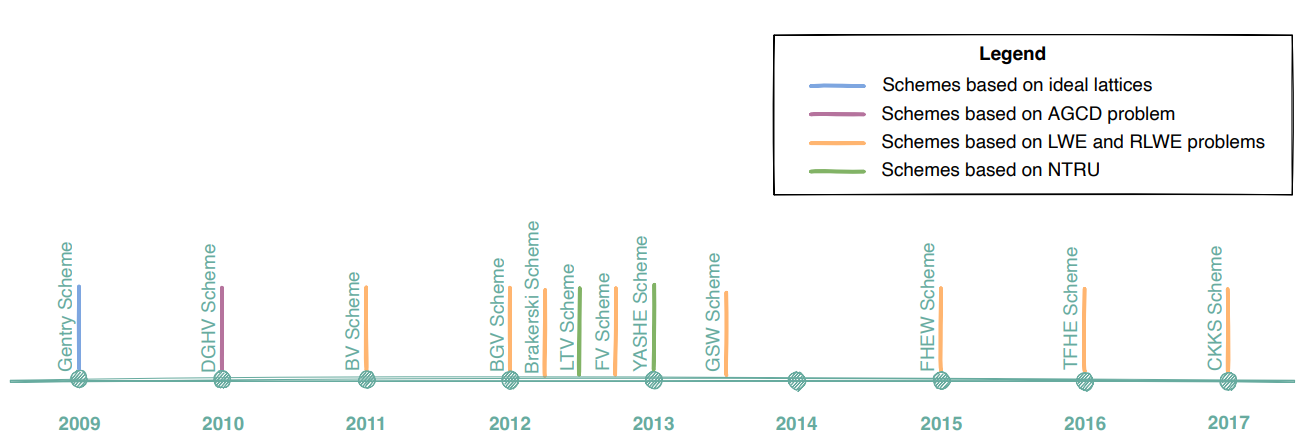
\includegraphics[scale=0.45]{bilder/FHE-Timeline.png}
  \caption{FHE Zeitlinie \cite{FHESurvey}}
  \label{fig:FheTimeline}
\end{figure}

Danach folgten mehrere Versuche dieses System zu verbessern, wie das 2011 erschiene BGV schema \cite{BGV} und das 2012 erschiene FV schema \cite{FV}. Beide Systeme sind LWE/RLWE basiert und unterscheiden sich im wesentlichen in der art und weise, wie sie mit dem wachsenden Fehler, vor allem bei der Multiplikation umgehen und diesen wieder reduzieren. Es folgten weitere Entwicklungen (siehe \ref{fig:FheTimeline}), aber auch Schwachstellen, wie die 2020 entdeckten Schwachstellen für CKKS \cite{SecurtyCKKS}.

Neben der Entwicklung neuer FHE-Schemas wurden auch versucht die bereits verfügbaren effizient zu Implementieren  \cite{FheImplementations}. Jedoch sind alle bisherigen FHE-Schemas schon von sich aus sehr ineffizient, wodurch es kaum praktische Einsätze dieser gibt.

Um dieses Problem zu lösen wird auch schon länger daran geforscht, FHE-Schemas direkt in Hardware umzusetzen und somit effizienter laufen zu lassen \cite{FheHardware2014} \cite{FheHardware2023}. 

\chapter{Vorgehensweisen und Methoden}
\label{VorgehensweisenUndMethoden}
Vorgehensweisen und Methoden
\chapter{Gliederung}
\label{Gliederung}
Gliederung
\chapter{Zeitplan}
\label{Zeitplan}

\begin{tabular}{|c | p{10cm} |}
  \toprule
  \multicolumn{2}{|l|}{$\mathbf{Vorbereitungen - Januar+Februar}$}                               \\
  \midrule
  Abgabe Expose bis          & 31.01.2020                                                        \\
  Einreichung Thema          & Mitte März 2020                                                   \\
  Literaturrecherche         & Sammlung von Literatur und Ausbauen der Mathematischen Grundlagen \\
  \midrule
  \multicolumn{2}{|l|}{$\mathbf{Ausarbeitung~Theoretischer~Teil - M"arz~bis~Mai}$}                \\
  \midrule
  Mathematische Ausarbeitung & Ausarbeitung der Mathematischen Grundlagen                        \\
                             & Entwicklung eines FHE-Schemas auf Basis von MLWE                  \\
  \midrule
  \multicolumn{2}{|l|}{$\mathbf{Ausarbeitung~Praktischer~Teil - Juni~bis~August}$}               \\
  \midrule
  Implementierung der Tests  & Ausarbeiten des Testkonzepts                                      \\
                             & Implementierung der Algorithmen                                   \\
                             & Ausarbeitung des Vergleichs                                       \\
  \midrule
  \multicolumn{2}{|l|}{$\mathbf{Abschluss - September}$}                                         \\
  \midrule
  Korrektur                  & Korrekturlesen                                                    \\
                             & Layout fertigstellen                                              \\
  \midrule
  \multicolumn{2}{|l|}{$\mathbf{Abgabe:~Ende~September}$}                                         \\
  \bottomrule                                                    
\end{tabular}


% ===============
%  Verzeichnisse
% ===============

% Verzeichnisse mit einzeiligem Zeilenabstand
\singlespacing

% Literaturverzeichnis
\listofreferences

% falls ein anderer Glossar-Stil genutzt wird und die zweite Spalte zu schmal ist:
% \setlength{\glsdescwidth}{0.8\linewidth}

% Glossar einfügen
\printglossary

% Index einfügen
\printindex

% wieder auf 1½-fachen Zeilenabstand umschalten
\normalspacing

\end{document}
